%%%%%%%%%%%%%%%%%%%%%%%%%%%%%%%%%%%%%%%%%%%%%%%%%%%%%%%%%%%%%%%%%%%%%%%%%%%%%
%	E-Yantra, IIT-Bombay

%	Document Author: Bhumika Varshney
%	Date: 30th June,2015

%%%%%%%%%%%%%%%%%%%%%%%%%%%%%%%%%%%%%%%%%%%%%%%%%%%%%%%%%%%%%%%%%%%%%%%%%%%%%
\documentclass[10pt,red]{beamer} 
% change the alerted colour to blue
\setbeamercolor{alerted text}{fg=blue}

\usetheme{berlin}
% theme split
\usepackage{beamerthemesplit}

% theme shadow
\usepackage{beamerthemeshadow}

% For including figures
\usepackage{graphicx}
\usepackage{booktabs,array}
\usepackage{listings}
\usepackage{hyperref}
\usepackage{verbatim,moreverb}
%\usepackage{tikz}
\usepackage{colortbl}
\usepackage{multirow}
% logo
\logo{
\includegraphics[height=1cm]{iitblogo.pdf}}


% sf family, bold font
\sffamily \bfseries
% Beginning of title page
\title
% content inside [] appears at bottom of all page. content inside {} appears on first page as title. double backslash means line change 
[
	Firebird LPC2148 Robotics Research Platform	% bottom
	\hspace{0.5cm}
	\insertframenumber/\inserttotalframenumber
]
{
	DC Motor Velocity Control \\Using Pulse Width Modulation (PWM)
}

\author
[
	www.e-yantra.org
]
{
	e-Yantra Team \\[20pt]
  Embedded Real-Time Systems Lab\\
  Indian Institute of Technology-Bombay \\
}
\date
{
IIT Bombay \\ {\today}
}
 
 
\begin{document}  

%Slide-1 for title page
\begin{frame}
   \titlepage
\end{frame}

%Slide-2 Content & Agenda for Talk 
\section*{outline}
\begin{frame}
	\frametitle{Agenda for Discussion}
	\tableofcontents
\end{frame}

\section{Introduction}
\subsection{Pulse Width Modulation}
%Slide-3
\begin{frame}
	\frametitle{Pulse Width Modulation} \pause
		\begin{enumerate}
			\item<+-|alert@+> Pulse Width Modulation (PWM), is a method of transmitting information on a series of pulses \\[10pt]
			\item<+-|alert@+> The data that is being transmitted is encoded on the width of these pulses to control the amount of power being sent to a load \\[10pt]
			\item<+-|alert@+> Examples: Electric stoves, Lamp dimmers, and Robotic Servos \\[10pt]
		\end{enumerate} \pause
		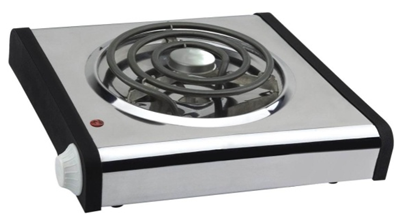
\includegraphics[width = 0.5\linewidth]{electric_stove} 
\end{frame}

\subsection{Duty Cycle}
%Slide-4
\begin{frame}[shrink = 2]
	\frametitle{Duty Cycle} \pause
		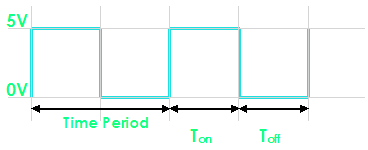
\includegraphics[width = \linewidth]{50_dutycycle} \pause
			\begin{enumerate}[$\checkmark$]
				\item<+-|alert@+> The signal remains "ON" for some time and  "OFF" for some time.
			 	\item<+-|alert@+> Ton = Time the output remains high.
			 	\item<+-|alert@+> Toff = Time the output remains Low.
			 	\item<+-|alert@+> When output is high the voltage is 5v
			 	\item<+-|alert@+> When output is low the voltage is 0v  
			 	\item<+-|alert@+> Time Period(T) = Ton + Toff
			 	\item<+-|alert@+> Duty Cycle = Ton*100/(Ton + Toff)
			  \item<+-|alert@+> Duty Cycle = 50\%
			\end{enumerate}
\end{frame}

%Slide-5
\begin{frame}[shrink = 2]
	\frametitle{Duty Cycle (Contd..)} \pause
		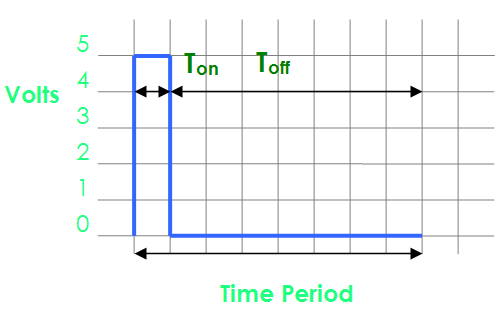
\includegraphics[width = \linewidth]{12_dutycycle} \pause
			\begin{enumerate}[$\checkmark$]
				\item<+-|alert@+> Ton = Time the output remains high = 1
			 	\item<+-|alert@+> Toff = Time the output remains Low = 7
			 	\item<+-|alert@+> Duty Cycle = 12.5\%
			\end{enumerate}
\end{frame}

%Slide-6
\begin{frame}[shrink = 2]
	\frametitle{Duty Cycle (Contd..)} \pause
		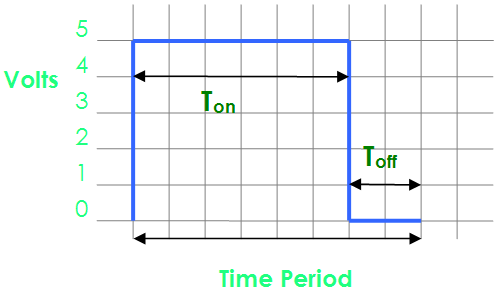
\includegraphics[width = \linewidth]{75_dutycycle} \pause
			\begin{enumerate}[$\checkmark$]
				\item<+-|alert@+> Ton = Time the output remains high = 6
			 	\item<+-|alert@+> Toff = Time the output remains Low = 2
			 	\item<+-|alert@+> Duty Cycle = 75\%
			\end{enumerate}
\end{frame}


\section{PWM Generation in AVR}
\subsection{Timer in AVR}
%Slide-7
\begin{frame}
	\frametitle{Timer in AVR} \pause
		\begin{enumerate}
		\item<+-|alert@+> The AVR microcontroller ATmega2560 has \\[10pt]
			\begin{itemize}[$\checkmark$]
				\item<+-|alert@+> two 8-bit timers (Timer0 and Timer2) and \\[10pt]
				\item<+-|alert@+> four 16-bit timers (Timer 1, 3, 4 and 5) \\[10pt]
			\end{itemize}
			
		\item<+-|alert@+>When the counter reaches its maximum count, it rolls over and executes from the start \\[10pt]
			\begin{itemize}[$\checkmark$]
				\item<+-|alert@+> For 8-bit counter, roll over occurs at 255 count and \\[10pt]
				\item<+-|alert@+> For 16-bit counter it occurs at 65535 count \\[10pt]
			\end{itemize}
		\end{enumerate}
\end{frame}

\subsection{Timer for PWM generation in Firebird}
%Slide-8
\begin{frame}
	\frametitle{Timer for PWM generation in Firebird} \pause
		\begin{enumerate}
			\item<+-|alert@+> Timer 5 can be used for PWM generation for controlling speed of motors \\[10pt]
			\item<+-|alert@+> The duty cycle of square wave generated by the Timer5 can be varied to produce different average DC values for motors\\[10pt]
			\item<+-|alert@+> Using FAST PWM mode to vary speed of motors\\[10pt]
		\end{enumerate}
\end{frame}

\section{PWM Generation in Firebird V}
\subsection{Registers}
%Slide-9
\begin{frame}
	\frametitle{Timer for PWM generation in Firebird} \pause
		\begin{enumerate}
			\item<+-|alert@+> To Program PWM, we have to initialize  some register before use it \\[10pt] 
			\item<+-|alert@+> Four registers are: \\[10pt]
			\begin{itemize}[number]	
				\item<+-|alert@+> TCCR5A \\[10pt]	 
				\item<+-|alert@+>	TCCR5B \\[10pt]
				\item<+-|alert@+>	TCNT5 \\[10pt] 	
				\item<+-|alert@+>	OCR5n \\[10pt]	
			\end{itemize}
		\end{enumerate}
\end{frame}

\subsection{TCCR5A}
%Slide-10
\begin{frame}
		\frametitle{TCCR5A- Timer Counter Control Register A} 
		\framesubtitle{This register is Used to Configure Timer for PWM generation}  \pause 
			%	\centering
				\begin{tabular}{!{\vrule width 0.8pt}>{\columncolor[gray]{0.9}[0.8\tabcolsep]}c|>{\columncolor[gray]{0.9}[0.8\tabcolsep]}c|>{\columncolor[gray]{0.9}[0.8\tabcolsep]}l|>{\columncolor[gray]{0.9}[0.8\tabcolsep]}c!{\vrule width 0.8pt}}
				\noalign{\hrule height 0.5pt}
				Bit & Symbol & Description & Bit Value  \\  
				\noalign{\hrule height 1pt} 
				\vspace{2pt} 
				7 & COM5A1 & Compare Output Mode for Channel A bit 1 & \color{red}  \textbf{1}\color{black} \\
				\vspace{2pt}
				6 & COM5A0 & Compare Output Mode for Channel A bit 0 &  0  \\
				\vspace{2pt}
				5 & COM5B1 & Compare Output Mode for Channel B bit 1 & \color{red}  \textbf{1}\color{black} \\
				\vspace{2pt}
				4 & COM5B0 & Compare Output Mode for Channel B bit 0 &  0 \\
				\vspace{2pt}
				3 & COM5C1 & Compare Output Mode for Channel C bit 1 & \color{red}  \textbf{1}\color{black} \\
				\vspace{2pt}
				2 & COM5C0 & Compare Output Mode for Channel C bit 0 &  0 \\
				\vspace{2pt}
				1 & WGM11 & Waveform Generation Mode bit 1 &  0 \\
				\vspace{2pt}
				0 & WGM10 & Waveform Generation Mode bit 0 & \color{red}  \textbf{1}\color{black} \\
				\noalign{\hrule height 0.5pt}			
			\end{tabular}	\pause \\[10pt]
		\hspace{8cm}TCCR5A\hspace{1pt}=\hspace{1pt}\color{red}0xA9 \color{black} 
\end{frame}

%Slide-11
\begin{frame}
		\frametitle{Compare Output Mode Fast PWM} \pause
			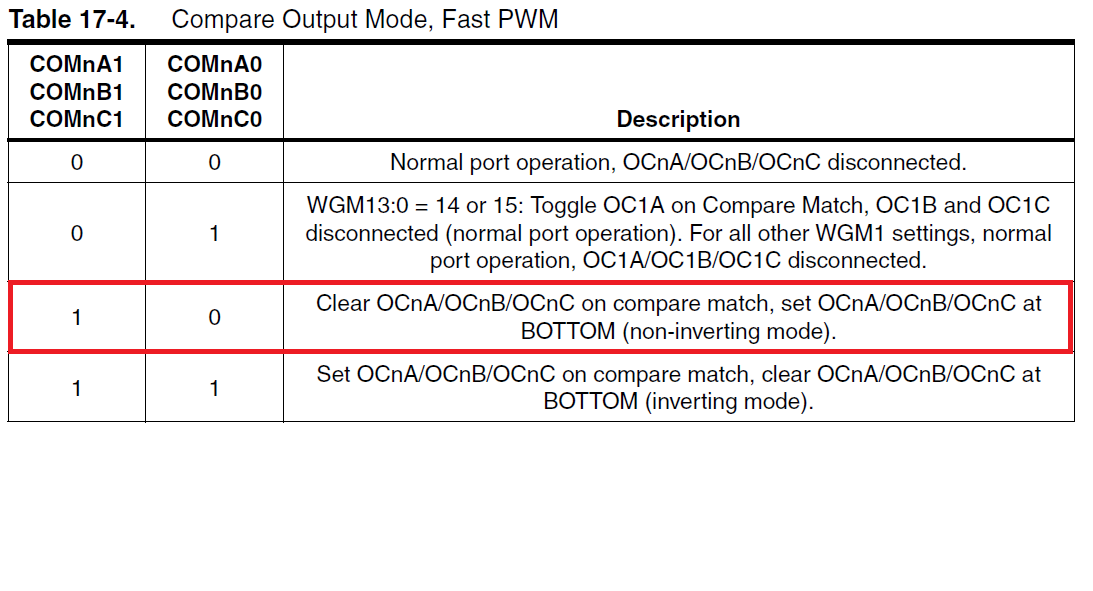
\includegraphics[width = \linewidth]{compare_output_mode_fastpwm}
\end{frame}

%Slide-12
\begin{frame}[shrink=5]
		\frametitle{Waveform Generation Bit} \pause
			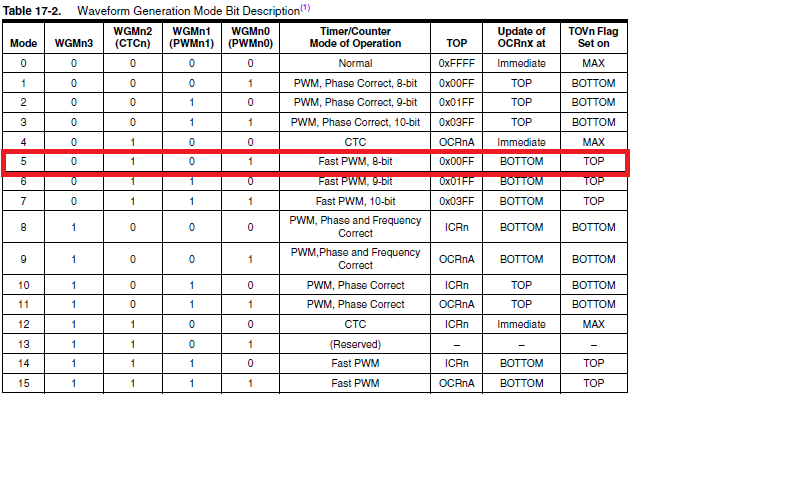
\includegraphics[width = \linewidth]{waveform_generation}
\end{frame}

\subsection{TCCR5B}
%Slide-13
\begin{frame}
		\frametitle{TCCR5B- Timer Counter Control Register B} 
		\framesubtitle{This register is Used to Configure Timer for PWM generation}  \pause 
			%	\centering
				\begin{tabular}{!{\vrule width 0.8pt}>{\columncolor[gray]{0.9}[0.8\tabcolsep]}c|>{\columncolor[gray]{0.9}[0.8\tabcolsep]}c|>{\columncolor[gray]{0.9}[0.8\tabcolsep]}l|>{\columncolor[gray]{0.9}[0.8\tabcolsep]}c!{\vrule width 0.8pt}}
				\noalign{\hrule height 0.5pt}
				Bit & Symbol & Description & Bit Value  \\  
				\noalign{\hrule height 1pt} 
				\vspace{2pt} 
				7 & ICNC5 & Input Capture Noise Canceller &  0  \\
				\vspace{2pt}
				6 & ICES5 & Input Capture Edge Select &  0  \\
				\vspace{2pt}
				5 & -- & Reserved Bit &   0 \\
				\vspace{2pt}
				4 & WGM53 & Waveform Generation Mode bit 3 &  0 \\
				\vspace{2pt}
				3 & WGM52 & Waveform Generation Mode bit 2 & \color{red}  \textbf{1}\color{black} \\
				\vspace{2pt}
				2 & CS52 & Clock Select &  0 \\
				\vspace{2pt}
				1 & CS51 & Clock Select & \color{red}  \textbf{1}\color{black}\\
				\vspace{2pt}
				0 & CS50 & Clock Select & \color{red} \textbf{1}\color{black} \\
				\noalign{\hrule height 0.5pt}			
			\end{tabular}	\pause \\[10pt]
		\hspace{8cm}TCCR5B\hspace{1pt}=\hspace{1pt}\color{red}0x0B \color{black} 
\end{frame}

%Slide-14
\begin{frame}
		\frametitle{Clock Select Bit} \pause
			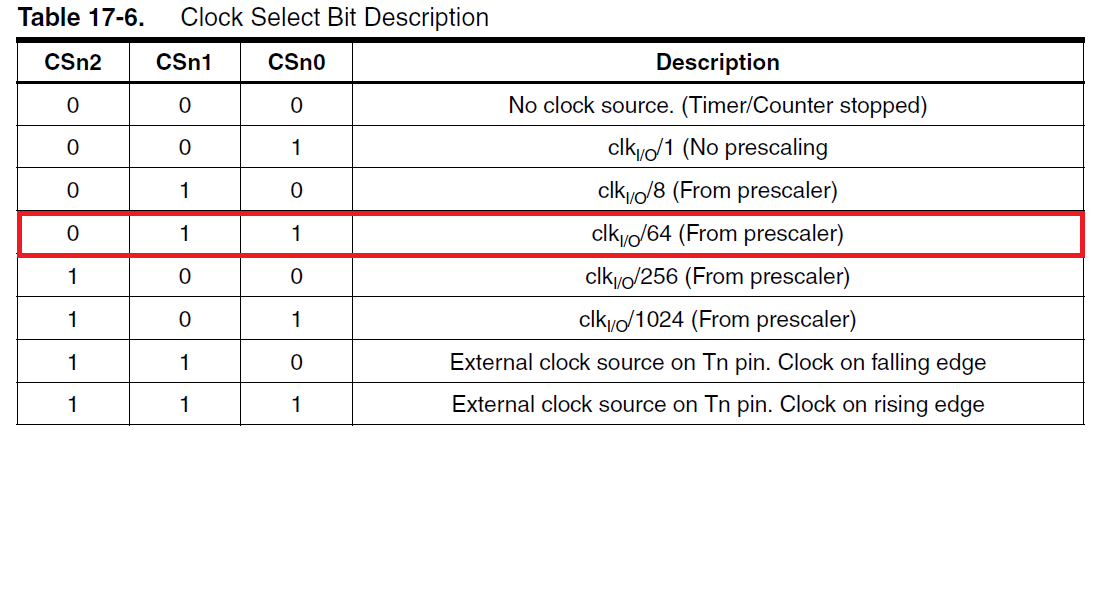
\includegraphics[width = \linewidth]{clock_select_bit} 
\end{frame}

\subsection{TCNT5}
%Slide-15
\begin{frame}
		\frametitle{TCNT5 : Timer/Counter5} \pause
			\begin{itemize}
				\item<+-|alert@+> Purpose: Counts Up/down according to clock frequency \\[10pt]
				\item<+-|alert@+> TCNT5 is a 16-bit Register  \\[10pt]
				\item<+-|alert@+> Counts from 0 to 255 if used in 8-Bit Mode \\[10pt]
				\item<+-|alert@+> Counts from 0 to 65535 if used in 16-Bit Mode \\[10pt]
			\end{itemize}
\end{frame}	

\subsection{OCR5}
%Slide-16
\begin{frame}
		\frametitle{Output Compare Register 5} \pause
			\begin{itemize}
				\item<+-|alert@+> Purpose: Compares itself from TCNT counter and set flags when match occurs \\[10pt]
				\item<+-|alert@+> OCR5n: where n=A/B/C are three different 16-bit Register  \\[10pt]
				\item<+-|alert@+> Each can be used individually as separate PWM channel \\[10pt]
				\item<+-|alert@+> OCR5n is represented as two 8-bit register as OCR5nL and OCR5nH \\[10pt]
				\item<+-|alert@+> PWM generated is 8-bit, so only lower register is used \\[10pt]
				\item<+-|alert@+> OCR5AL (PortL3) is connected to Left Motor  \\[10pt]
				\item<+-|alert@+> OCR5BL (PortL4) is connected to Right Motor \\[10pt]
			\end{itemize}
\end{frame}	

%Slide-17
\begin{frame}
		\frametitle{Output Compare Register 5 (Contd..)} \pause
			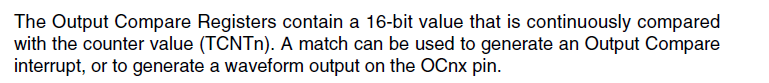
\includegraphics[width = \linewidth]{ocr5_1} \pause \\[20pt]
			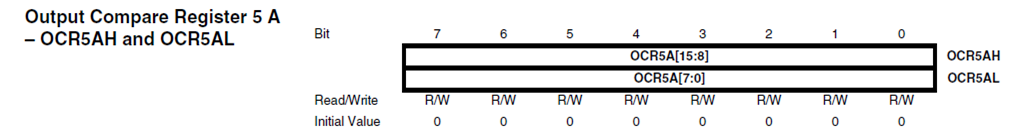
\includegraphics[width = \linewidth]{ocr5_2}  \\[10pt]
\end{frame}

\subsection{Block Diagram}
%Slide-18
\begin{frame}
		\frametitle{Block Diagram - Output Compare Unit} \pause
			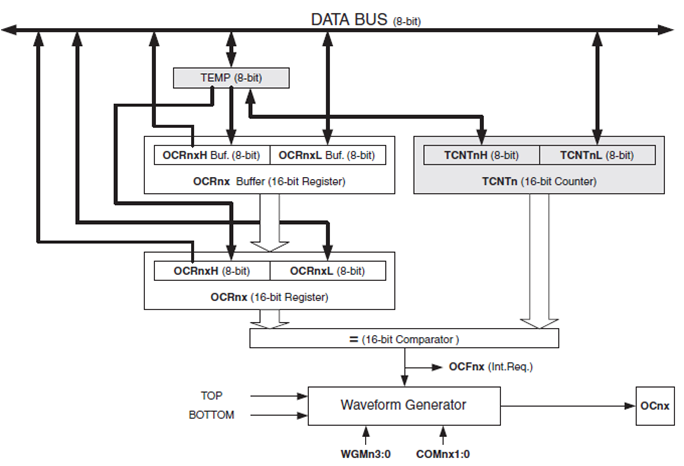
\includegraphics[width = \linewidth]{block_diagram_output_compare_unit} 	
\end{frame}

%Slide-19
\begin{frame}
		\frametitle{Timing Diagram Fast PWM} \pause
			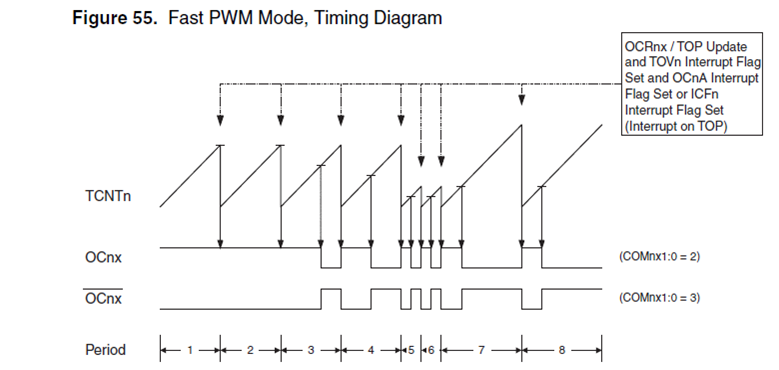
\includegraphics[width = \linewidth]{Timing_diagram_fast_PWM} 	
\end{frame}

\subsection{Program}
%Slide-20
\begin{frame}[shrink = 4,fragile]
	\frametitle{Syntax for C-Program} \pause
	\framesubtitle{PWM Initialization}
		\begin{block}<1->{Port Pin Config}	\pause
		\begin{semiverbatim}
				\scriptsize{
				void motion_pin_config (void) \color{green} //Configure Pins as Output\color{black}
				\{
					 
					 Port A for motion control and Port L for Velocity Control must be defined Output
					 
				\} }
			\end{semiverbatim}
		\end{block} \pause
	
	\begin{block}<1->{PWM Initialization}	\pause
		\begin{semiverbatim}
				\scriptsize{
				void timer5_init()	\color{green} //Set Register Values for starting Fast 8-bit PWM  \color{black}
				\{
					 
  					TCCR5A =  
			\ \ \	TCCR5B =
			\ \ \	TCNT5H = 0xFF; 
			\ \ \	TCNT5L = 0x00; 
			\ \ \	OCR5AH = 0x00;
			\ \ \ OCR5AL = 0xFF;
			\ \ \	OCR5BH = 0x00;
			\ \ \ OCR5BL = 0xFF;
				\} }
			\end{semiverbatim}
		\end{block} 
\end{frame}

%Slide-21
\begin{frame}[shrink = 2,fragile]
	\frametitle{Syntax for C-Program} \pause
	\framesubtitle{Program}
		\begin{block}<1->{Main Program}	\pause
		\begin{semiverbatim}
				\scriptsize{
				int main(void)
				\{
			\ \		init_devices(); 
			\ \		forward();
			\ \		while(1)
			\ \		\{
			\ \ \ \			velocity(100,100);
			\ \ \ \			_delay_ms(500);
			\ \ \ \			velocity(0,255);
			\ \ \ \			_delay_ms(500);
			\ \		\}
				\}
 }
			\end{semiverbatim}
		\end{block} \pause
	
	\begin{block}<1->{Velocity Function}	\pause
		\begin{semiverbatim}
				\scriptsize{
				void velocity (unsigned char left_motor, unsigned char right_motor)	
				\{
					 
			  		OCR5AL = (unsigned char)left_motor;
			\ \ \	OCR5BL = (unsigned char)right_motor;
				\}} 
			\end{semiverbatim}
		\end{block} 
\end{frame}

%Slide-22		
\begin{frame}
\hskip4cm
\textbf{\LARGE Thank You!} \\[20pt]
\hskip3cm
\scriptsize Post your queries on: 
\hyperref[www.e-yantra.org]{\color{blue} http://qa.e-yantra.org/ \color{black}} 
\end{frame}
\end{document}

